\documentclass[11pt]{article}
% \usepackage{ctex}
\usepackage{geometry}
\usepackage{amsmath,amsfonts,graphicx,amssymb,bm,amsthm}
\usepackage{mathtools}
\usepackage{mathrsfs}
\usepackage[square, numbers]{natbib}
\bibliographystyle{abbrv}
\usepackage{lastpage}
\usepackage{paralist}
\usepackage{booktabs}
\usepackage[colorlinks]{hyperref}
\geometry{left=3.17cm, right=3.17cm, top=2.54cm, bottom=2.54cm} % A4纸
\usepackage{fancyhdr}
\usepackage{graphicx}
\usepackage{float}
\usepackage{xcolor}
\usepackage{listings} % 代码
% 替换部分符号
\DeclareSymbolFont{CMlargesymbols}{OMX}{cmex}{m}{n}
\let\sumop\relax\let\prodop\relax
\DeclareMathSymbol{\sumop}{\mathop}{CMlargesymbols}{"50}
\DeclareMathSymbol{\prodop}{\mathop}{CMlargesymbols}{"51}
% 代码高亮
\lstset{
    language=C++,
    numberstyle=\tiny,
    basicstyle=\small\ttfamily,
    stringstyle=\color{purple},
    keywordstyle=\color{blue}\bfseries,
    commentstyle=\color{olive},
    directivestyle=\color{blue},
    frame=single,
    rulesepcolor=\color{red!20!green!20!blue!20}
}
\usepackage{algorithm2e}
% \usepackage{algorithm,algorithmicx}


\usepackage{comment}
\usepackage{diagbox}
\usepackage[noend]{algpseudocode}
\usepackage{fontspec}
\usepackage{longtable}
\usepackage{newclude}
%Includes "References" in the table of contents
\usepackage[nottoc]{tocbibind}

% write inference rules
\usepackage{proof}
\usepackage{semantic}
\usepackage{mathpartir}
\usepackage{authblk}
\usepackage{multicol}
% \setmonofont{Fira Code}
% \setsansfont[BoldFont={Fira Sans Medium}]{Fira Sans Light}
\newfontfamily{\lstfont}[Scale=.85]{Fira Sans}

\newtheorem{Def}{Definition}
\newtheorem{Thm}{Theorem}
\newtheorem{Prop}{Proposition}
\newtheorem{Proof}{Proof}

\setmainfont{Times}
% \usepackage{unicode-math}
% \setmathfont{STIX Two Math}
% 字体更换
% \usepackage{newtxtext}
% \usepackage{newtxmath}

\usepackage{listings}
\definecolor{light-gray}{gray}{0.85}
\lstdefinelanguage{lambda}{%
  morekeywords={%
    if,then,else,fix,fun % keywords go here
  },%
  morekeywords={[2]Nat,Bool,Vector},   % types go here
  otherkeywords={}, % operators go here
  literate={% replace strings with symbols
    {<-}{{$\from$}}{2}
    {<-|}{{$\hookleftarrow$}}{2}
    {->}{{$\to$}}{2}
    {lambda}{{$\lambda$}}{1}
    {/}{{$\kappa$}}{1}
  },
  basicstyle={\lstfont}, 
  keywordstyle={\bfseries},
  keywordstyle={[2]\itshape}, % style for types
  keepspaces,
  mathescape, 
  columns=fixed,
  backgroundcolor = \color{light-gray}
}[keywords,comments,strings]

\usepackage{titling}% the wheel somebody else kindly made for us earlier
\pretitle{% add some rules
  \begin{center}
    \fontsize{20}{22}\bfseries
}%, make the fonts bigger, make the title (only) bold
\posttitle{%
  \end{center}%
  \noindent\vrule height 1.5pt width \textwidth
  \vskip .75em plus .25em minus .25em% increase the vertical spacing a bit, make this particular glue stretchier
}

\usepackage{titlesec}
\titleformat{\section}
  {\normalfont\fontsize{14}{17}\sffamily\bfseries}
  {\thesection}{1em}{}
\titleformat{\subsection}
  {\normalfont\fontsize{12}{17}\sffamily\bfseries\slshape}
  {\thesubsection}{1em}{}
\titleformat{\subsubsection}
  {\normalfont\fontsize{11}{17}\sffamily\bfseries\slshape}
  {\thesubsubsection}{1em}{}

\newcommand{\mycomment}[2]{{\small\color{magenta}\underline{\sf{#1}}:} {\color{magenta}{\small #2}}}

\title{$\bm{\lambda_Q}$ : A Simple Quantum Programming Language}
\author{
  Wenhao Tang\quad \texttt{1800013088}
  % \texttt{first1.last1@xxxxx.com}
  \\[1ex]
  Xinzhao Wang\quad \texttt{1800013102}
  % \texttt{first2.last2@xxxxx.com}
}
\affil{Department of EECS\\ Peking University}
\date{\today}

\fancypagestyle{plain}{
	\lhead{\small $\lambda_Q$ : A Simple Quantum Programming Language}
	\chead{}
	\rhead{}
	\lfoot{\small Wenhao Tang, Xinzhao Wang}
	\cfoot{}
	\rfoot{\thepage\ / \ \pageref*{LastPage} }
}
\pagestyle{plain}

\renewcommand{\headrulewidth}{0.4pt}
\renewcommand{\footrulewidth}{0.4pt}

\begin{document}

\maketitle
\tableofcontents

\renewcommand{\t}{\mathtt{t}}

\newcommand{\true}{\mathtt{true}}
\newcommand{\false}{\mathtt{false}}
\newcommand{\tif}{\mathtt{if}}
\newcommand{\tthen}{\mathtt{then}}
\newcommand{\telse}{\mathtt{else}}
\newcommand{\unit}{\mathtt{unit}}
\newcommand{\Unit}{\mathtt{Unit}}
\newcommand{\One}{\mathtt{1}}
\newcommand{\Bool}{\mathtt{Bool}}
\newcommand{\Bit}{\mathtt{Bit}}
\newcommand{\Qubit}{\mathtt{Qubit}}
\newcommand{\trun}{\mathtt{run}}
\newcommand{\toutput}{\mathtt{output}}
\newcommand{\from}{\leftarrow}
\newcommand{\From}{\Leftarrow}
\newcommand{\To}{\Rightarrow}
\newcommand{\gate}{\mathtt{gate}}
\newcommand{\lift}{\mathtt{lift}}
\newcommand{\capp}{\mathtt{capp}}
\newcommand{\calG}{\mathcal{G}}
\newcommand{\new}{\mathtt{new}}
\newcommand{\init}{\mathtt{init}}
\newcommand{\meas}{\mathtt{meas}}
\newcommand{\discard}{\mathtt{discard}}
\newcommand{\Ha}{\mathtt{H}}
\newcommand{\X}{\mathtt{X}}
\newcommand{\Z}{\mathtt{Z}}
\newcommand{\CNOT}{\mathtt{CNOT}}


\newcommand{\ccc}{\color[rgb]{0.5,0.11,0.1}}

\section{Introduction}
Quantum computing is getting more and more popular these days.
\mycomment{twh}{Add some background of quantum computing here @wxz.}
blah\\
blah\\
blah\\
blah\\
blah\\

There are three main models of quantum computing: \textit{Quantum Turing Machine}, \textit{Quantum $\lambda$-Calculus} and \textit{Quantum Circuit}, among which the third one is the most practical.
Most quantum programming languages are \textit{quantum-circuit description languages}, which means they are used to describe the architecture of quantum circuits.
The current quantum programming languages can be categorized into two categories according to their styles: functional quantum programming languages and imperative quantum programming languages.
\begin{multicols}{2}
  \begin{center}
      Functional:
  \end{center}
\begin{itemize}
    \item Qwire
    \item QML
    \item Quipper
    \item QuaFL
    \item Silq
\end{itemize}

  \columnbreak

  \begin{center}
          Imperative:
  \end{center}
\begin{itemize}
    \item QASM
    \item QCL
    \item ScaffCC
    \item Qiskit
    \item Quil
\end{itemize}
\end{multicols}

Advanced quantum programming languages can use more powerful abstract constructs and type systems to make it easier for programmers to write correct quantum programs.
In particular, we design a simple quantum programming language named $\lambda_Q$, which means \textbf{$\boldsymbol{\lambda}$-calculus with quantum circuit}.
Its syntax consists of a traditional part, which is a simple $\lambda$-calculus, and a quantum part, whose syntax is based on Qwire, a functional quantum programming language with linear type system.
What's more, we implement a compiler from $\lambda_Q$ to QASM (Quantum Assembly Language), an imperative quantum programming language with low-level instruction sets.
The output QASM program can run on the IBM cloud quantum machine.

The main feature of $\lambda_Q$ is that the syntax for traditional computation and quantum computation are separated.
They communicate with each other via some specific operations : quantum circuit can be \textit{abstracted} or \textit{lifted (measured)} into traditional term, and traditional term for quantum circuit can be applied to quantum bits.
Thus, the syntax of quantum circuit can use \textit{linear type system} to guarantee that the Quantum Non-cloning Theorem is not violated, meanwhile the $\lambda$-calculus of the traditional part makes it easier to write quantum programs.
We will explain it in detail in Section \ref{spec}.

The overall structure of the compiler can be visualized in Figure \ref{compiler}.
The frontend is implemented using \texttt{Haskell}, and the backend is implemented using \texttt{C}.
The code can be found in \url{https://github.com/thwfhk/lambdaQ}.
We will discuss the implementation of $\lambda_Q$ compiler in detail in Section \ref{front} and \ref{back}.


\begin{center}
  \begin{figure}
    \label{compiler}
    \centering
    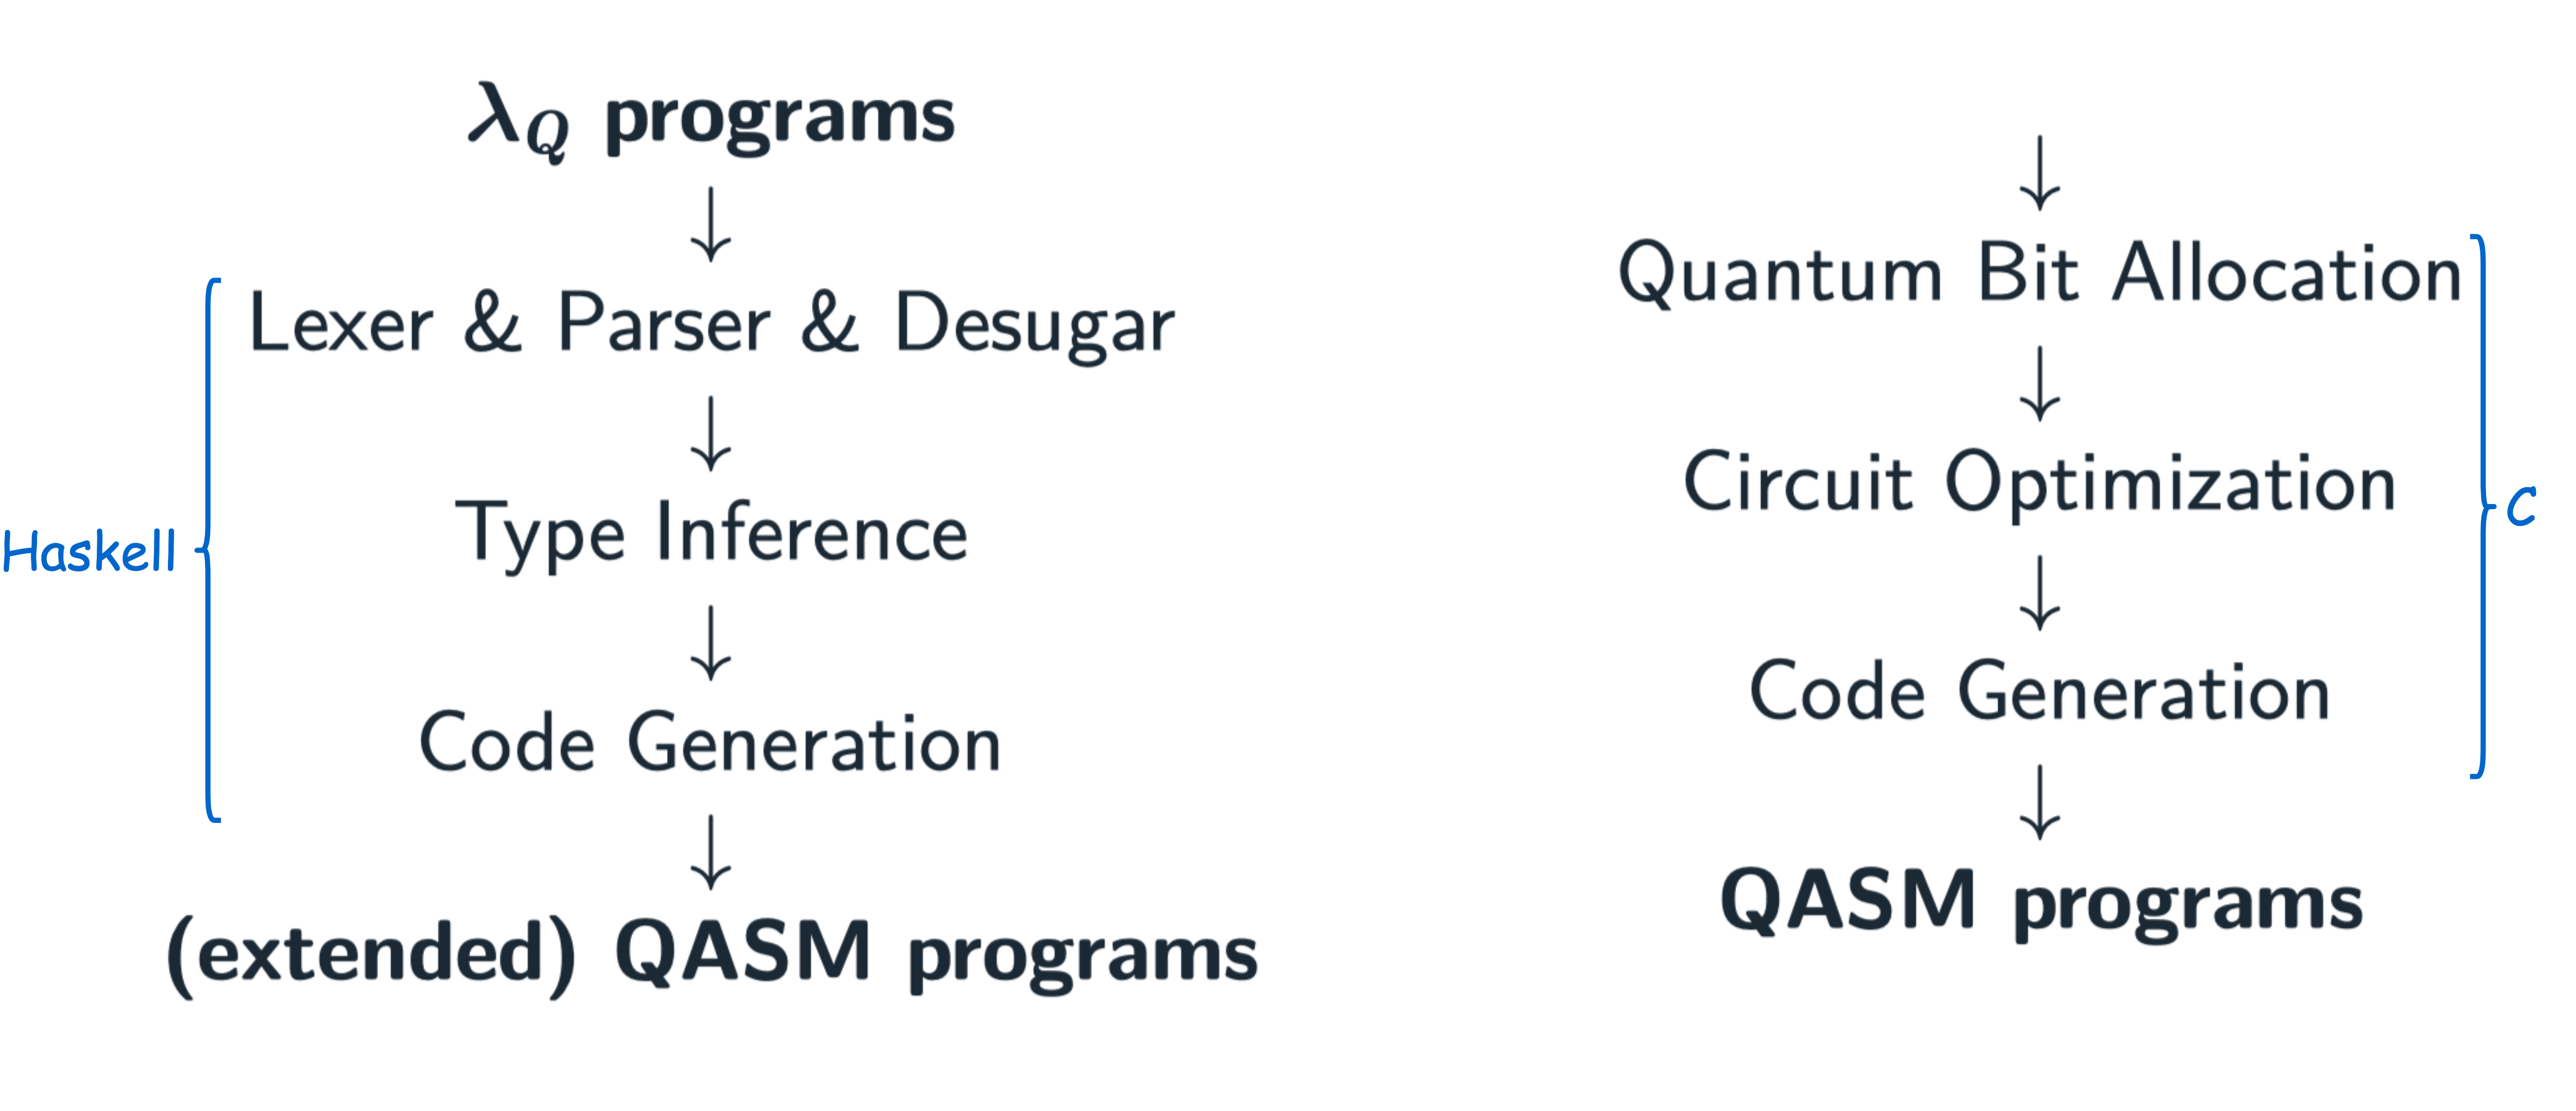
\includegraphics[width=0.9\linewidth]{images/overview.png}
    \caption{Structure of $\lambda_Q$ compiler.}
  \end{figure}
\end{center}

\section{Specification of $\lambda_Q$} \label{spec}

In this section we give the language specification of $\lambda_Q$, including the syntax, typing rules and syntactic sugars.
The syntax and typing rules of the quantum circuit are similar to Qwire \cite{qwire}.
The operational semantics are not given in this section.
Instead, we give a transformation from $\lambda_Q$ to $QASM$ in the section of frontend, which gives semantics to each syntax of $\lambda_Q$.
Interested readers can refer to the operational semantics of simply-typed $\lambda$-calculus and Qwire.

\subsection{Syntax}
The syntax of the traditional part (terms, values, types) is an extended version of simply-typed $\lambda$-calcus with $\trun\ C$ and $\kappa \ p:W . C$, which are used to interact with the quantum part.
The syntax of the quantum part (circuits, wire types, wire patterns, gates, gate types) is similar to the syntax of Qwire.
% \mycomment{twh}{modify syntax (especially gate)}

\begin{longtable}[c]{lclr}
  % \caption{syntax}
  \label{tab:table1}\\
  \toprule
  $t$ &$::=$ &  &\textbf{terms}: \\
      & &$x$ &variable\\
      & &$\unit$ &constant unit\\
      & &$\true$ &constant true\\
      & &$\false$ &constant false\\
      & &$\lambda\ x:T.t$ &function abstraction\\
      & &$t\ t$ &function application\\
      & &$(t, t)$ &pair\\
      & &$t.1$ &first projection\\
      & &$t.2$ &second projection\\
      & &$\tif\ t\ \tthen\ t\ \telse\ t$ &conditional\\
      & &$\trun\ C$ &static lifting\\
      & &$\kappa \ p:W . C$ &circuit abstraction\\
      % & &0 &constant zero\\
      % & &succ $t$ &successor\\
      % & &pred $t$ &predecessor\\
      % & &iszero $t$ & zero test\\
  \\
  
  $v$ &$::=$ &  &\textbf{values}: \\
      & &$\lambda\ x:T.t$ &abstraction value\\
      & &$(v, v)$ &pair value\\
      & &$\unit$ &unit value\\
      & &$\true$ &true value\\
      & &$\false$ &false value\\
      & &$\kappa\ p:W . C$ &circuit value\\
  \\

  $T$ &$::=$ &  &\textbf{types}: \\
      & &$\Unit$ &unit type\\
      & &$\Bool$ &boolean type \\
      & &$T\times T$ &product type\\
      & &$T\to T$ &function type\\
      & &$T\leadsto T$ &circuit type\\
      % & &Nat &type of natural numbers\\
      % & &Vector $t$ &type family of vectors\\
  \\

  $\Gamma$ &$::=$ &  &\textbf{contexts}: \\
      & &$\varnothing$ &empty context\\
      & &$\Gamma,x:T$ &term variable binding\\
  \\


  $W$ &$::=$ &  &\textbf{wire types}: \\
      & &$\One$ &wire unit type\\
      & &$\Bit$ &bit type \\
      & &$\Qubit$ &qubit type \\
      & &$W \otimes W$ &wire product type \\
  \\

  $p$ &$::=$ &  &\textbf{wire patterns}: \\
      & &$()$ &empty\\
      & &$w$ &wire variable \\
      & &$(p,p)$ &wire pair \\
  \\

  $C$ &$::=$ &  &\textbf{circuits}: \\
      & &$\toutput\ p$ &output a pattern \\
      & &$p_2 \from \gate\ g\ p_1 ; C$ &gate application \\
      & &$p \from C ; C$ &circuit composition \\
      & &$x \hookleftarrow \lift\ p ; C$ &dynamic lifting \\
      & &$\capp\ t\ \mathtt{to}\  p$ &circuit application \\
  \\

  $g$ &$::=$ &  &\textbf{gates}: \\
      & &$\new_0$ &generate a bit 0 \\
      & &$\new_1$ &generate a bit 1 \\
      & &$\init_0$ &generate a qubit 0 \\
      & &$\init_1$ &generate a qubit 1 \\
      & &$\meas$ &measurement gate \\
      & &$\discard$ &disgard gate \\
      & &$\Ha$ &Hadamard gate \\
      & &$\X$ &Pauli-X gate \\
      & &$\Z$ &Pauli-Z gate \\
      & &$\CNOT$ &CNOT gate \\
  \\

  $G$ &$::=$ &  &\textbf{gate types}:\\
      & &$\mathcal{G}(W, W)$ &simple gate type\\
  \\

  $\Omega$ &$::=$ &  &\textbf{wire contexts}: \\
      & &$\varnothing$ &empty context\\
      & &$\Omega,w:W$ &wire variable binding\\
  \\
  % TODO: add the condition of well-formed contexts

  \bottomrule
  
\end{longtable}

\subsection{Typing Rules} \label{typing}
The main feature of the language design of $\lambda_Q$ is to use linear type system to guarantee no quantum bit is used twice or not used at all.
To state the type inference rules of $\lambda_Q$, we first need to define what is a \textbf{well-formed wire context}, which is used to maintain variables used by quantum circuit in the calculus.
This context is actually corresponding to the context of linear variables in the traditional linear type system.
\begin{Def}[Well-formed Wire Contexts]
  A wire context $\Omega$ is well-formed, if there are no duplicate wire variables in it.
  For simplicity, we always assume the wire contexts are well-formed in the following contexts. And when we write $\Omega_1, \Omega_2$, we require $\Omega_1$ and $\Omega_2$ to be disjoint to preserve the well-formedness.
\end{Def}

Since there are some different kinds of terms: ($\lambda$-)terms, wire patterns, gates and circuits, we have defined several different typing relations for each of them.
\begin{itemize}
  \item $\Omega \vdash p : W$ is the typing relation for patterns.
  \item $\Gamma ; \Omega \vdash C : W$ is the typing relation for circuits;
  \item $\Gamma \vdash t:T$ is the typing relation for ($\lambda$-)terms;
  \item $g : G$ is the typing relation for gates.
\end{itemize}

\subsubsection{Typing rules for gates}
Note that since we only support built-in gates, the typing rules for gates are extremely simple, just assigning a type to each built-in gate.

\noindent \textbf{Typing rules for gates}: $\boxed{g : G}$
\renewcommand\arraystretch{2.5}
\begin{longtable}[c]{cr}
  $ \infer{\new_0 : \calG(\One, \Bit)}{}$ & \\
  $ \infer{\new_1 : \calG(\One, \Bit)}{}$ & \\
  $ \infer{\init_0 : \calG(\One, \Qubit)}{}$ & \\
  $ \infer{\init_1 : \calG(\One, \Qubit)}{}$ & \\
  $ \infer{\meas : \calG(\Qubit, \Bit)}{}$ & \\
  $ \infer{\discard : \calG(\Bit, \One)}{}$ & \\
\end{longtable}

\subsubsection{Typing rules for patterns}
The patterns are used to construct complex gates.
Patterns are destructed when doing pattern matching in gate application, circuit composition and dynamic lifting.

\noindent \textbf{Typing rules for patterns}: $\boxed{\Omega \vdash p : W}$
\renewcommand\arraystretch{2.5}
\begin{longtable}[c]{cr}
  $ \infer{\varnothing \vdash ():One}{}$ & \\
  $ \infer{w:W \vdash w:W}{}$ & \\
  $ \infer{\Omega_1, \Omega_2 \vdash (p_1,p_2):W_1\otimes W_2}{\Omega_1 \vdash p_1 : W_1  &\Omega_2 \vdash p_2 : W_2} $ & \\
\end{longtable}

\subsubsection{Typing rules for circuits}
The typing rules for circuit uses linear type. The context $\Gamma$ is for normal (traditional) variables and the context $\Omega$ is for linear (quantum) variables.

\noindent \textbf{Typing rules for circuits}: $\boxed{\Gamma;\Omega\vdash C:W}$


\renewcommand\arraystretch{3} 
\begin{longtable}[c]{cr}
  $\infer{\Gamma;\Omega\vdash \toutput\ p:W}{\Omega\vdash p : W}$ &(C-OUTPUT)\\
  $\infer{\Gamma;\Omega_1,\Omega\vdash p_2 \from \gate\ g\ p_1 ; C:W}{g:\calG(W_1, W_2) &\Omega_1\vdash p_1:W_1 &\Omega_2\vdash p_2:W_2 &\Gamma ; \Omega_2,\Omega \vdash C:W}$ &(C-GATE)\\
  $\infer{\Gamma;\Omega_1,\Omega_2\vdash p \from C ; C':W'}{\Gamma;\Omega_1\vdash C:W &\Omega \vdash p:W &\Gamma;\Omega,\Omega_2 \vdash C':W'}$ &(C-COMPOSE)\\
  $\infer{\Gamma;\Omega,\Omega'\vdash x \hookleftarrow \lift\ p ; C:W'}{\Omega\vdash p:W &\Gamma,x:|W|;\Omega' \vdash C:W'}$ &(C-LIFT)\\
  $\infer{\Gamma;\Omega\vdash \capp\ t\ \mathtt{to}\ p : W_2}{\Gamma\vdash t:W_1\leadsto W_2 &\Omega\vdash p:W_1}$ &(C-CAPP)\\
  
\end{longtable}

\subsubsection{Typing rules for terms}

\noindent \textbf{Typing rules for ($\lambda$-)terms}: $\boxed{\Gamma\vdash t:T}$

\renewcommand\arraystretch{3}
\begin{longtable}[c]{cr}
  $\infer{\Gamma\vdash \trun\ C : |W| }{\Gamma;\varnothing \vdash C:W}$ &(T-RUN)\\
  $\infer{\Gamma\vdash \kappa\ p:W_1 . C: W_1\leadsto W_2 }{\Omega\vdash p:W_1 &\Gamma;\Omega\vdash C:W_2}$ &(T-CABS)\\
  $\infer{\Gamma\vdash x:T}{x:T\in \Gamma}$ &(T-VAR)\\
  $\infer{\Gamma\vdash \lambda\ x:T_1.t_2 : T_1\to T_2}{\Gamma,x:T_1 \vdash t_2:T_2}$ &(T-ABS)\\
  $\infer{\Gamma\vdash t_1\ t_2 : T_{12}}{\Gamma\vdash t_1:T_{11}\to T_{12} & \Gamma\vdash t_2:T_{11}}$ &(T-APP)\\
  $\infer{\Gamma\vdash\true : Bool}{}$ &(T-TRUE)\\
  $\infer{\Gamma\vdash\false : Bool}{}$ &(T-FALSE)\\
  $\infer{\tif\ t_1\ \tthen\ t_2\ \telse\ t_3 : T}{\Gamma\vdash t_1:\Bool &\Gamma\vdash t_2:T &\Gamma\vdash t_3:T}$ &(T-IF)\\
  $\infer{\Gamma\vdash\unit : Unit}{}$ &(T-UNIT)\\
  $\infer{\Gamma\vdash (t_1,t_2) : T_1\times T_2}{\Gamma\vdash t_1:T_1 &\Gamma\vdash t_2:T_2}$ &(T-PAIR)\\
  $\infer{\Gamma\vdash t.1 : T_1}{\Gamma\vdash t : T_1\times T_2}$ &(T-FST)\\
  $\infer{\Gamma\vdash t.2 : T_2}{\Gamma\vdash t : T_1\times T_2}$ &(T-SEC)\\
\end{longtable}

% \begin{longtable}[c]{cr}
%   $\infer{\Gamma\vdash x:T}{x:T\in\Gamma &\Gamma\vdash T::*}$ &(T-VAR)\\
%   $\infer{\Gamma\vdash \lambda x:S.t\ :\Pi x:S.T}{\Gamma\vdash S::* &\Gamma,x:S\vdash t:T}$ &(T-ABS)\\
%   $\infer{\Gamma \vdash t_1\ t_2 : [x\mapsto t_2]T}{\Gamma\vdash t_1:\Pi x:S.T &\Gamma\vdash t_2:S}$ &(T-APP)\\
%   $\infer{\Gamma\vdash (t_1,t_2:\Sigma x:S.T)\ :\Sigma x:S.T}{\Gamma \vdash t_1:S &\Gamma\vdash t_2:[x\mapsto t_1]T}$ &(T-PAIR)\\
%   $\infer{\Gamma\vdash t.1:S}{\Gamma\vdash t:\Sigma x:S.T}$ &(T-PROJ1)\\
%   $\infer{\Gamma\vdash t.2:[x\mapsto t.1]T}{\Gamma\vdash t:\Sigma x:S.T}$ &(T-PROJ2)\\
%   $\infer{\Gamma\vdash t:T'}{\Gamma\vdash t:T &\Gamma\vdash T\equiv T'::*}$ &(T-CONV)\\
% \end{longtable}

\subsection{Syntactic Sugar}
In programming languages, it is useful to design some syntactic sugar to make it easier for programmer to programming.
We introduce a syntactic sugar to $\lambda_Q$ to abstract one common form of gate application.
$$p \from \gate\ g\ p;\toutput\ p \ =\ \gate'\ g\ p$$

\section{Frontend}
In this section we illustrate the design and implementation of the frontend of compiler of $\lambda_Q$.

\subsection{Lexer \& Parser}

\subsection{Desugar}

\subsection{Type Inference}

\subsection{}

\section{Backend} \label{back}
In this section we illustrate the design and implementation of the backend of compiler of $\lambda_Q$.
The backend consists of four parts: lexer, parser, qubit allocation and optimization.
\subsection{Lexer \& Parser}
We use Lex/Yacc to implement the lexer and parser of a modified version of OpenQasm2.0 in backend.

Subcircuit definition is not available in our OpenQasm2.0. Besides $\{U3,CX\}$ that are available in the original OpenQasm2.0, we add $\{H,X,Y,Z\}$ to the built-in gate set.

This part consists of 600 lines of C code formatted in Lex/Yacc file's syntax.
Readers can refer to \textit{lex.l} and \textit{parser.y} to get more detailed information.

\subsection{Qubit allocation}
In recent years, some companies like IBM have made quantum computers available to wide community.
Users can build their experiments based on a circuit representation on the cloud platform. However, today's quantum computer prototypes have tight resources constraints.
For instance, you can only apply two qubits operations to a subset of qubit pairs which is specificed by a partial network.

In \textit{qubit\_allocation.cpp}, we implement a heuristic algorithm  to allocate physical qubits to logic qubits.

\subsubsection{Problem Definition}
The most basic form of Qubit Allocation Problem is: given a quantum circuit and an architecture, we want to know if it is possible to map logic qubits in the former to physical qubits in the latter.
Notice that even this basic form problem is already NP-hard.

In some cases, the constraints of the architecture is impossible to satisfy, and we need some circuit transformation to relax these constraints.

There are three kinds of transformation we can apply:
\begin{itemize}
    \item[Reversal] Apply $CX$ to $(p,q)$ when $(q,p)$ is available in the architecture.
    \item[Bridge] Apply $CX$ to $(p,q)$ when $(p,s)$ and $(s, q)$ is available.
    \item[Swap] Swap the state of $p$ and $q$ when $(p,q)$ or $(q,p)$ is available.
\end{itemize}

All these transformation need extra gates to implement, so we need to find a qubit mapping and circuit transformations to satisfy the constraints with minimum number extra gates involved.

\subsubsection{Algorithm}

Our algorithm has two stages:

\textbf{First stage}: Find an intial mapping

We first sort the logic qubits in descending order of their occurrence counts.

Then, for each logic qubit $q$ in order, we allocate $q$ to a physical qubit with the nearest out-degree(both the quantum circuit and the architecture can be regarded as a directed graph whose vertex is qubits)

After $q$ is allocated to $p$, for each edge $(q,q')$, we try to allocate $q'$ to some $p'$ with edge $(p,p')$ and has the nearest out-degree.

Repeat the above process for $q'$ if it is successfully allocated.

After this BFS-like allocation we allocate the rest unallocated logic qubit to a free physical qubit.

\textbf{Second stage}: Adjust the mapping and apply circuit transformation

The mapping $l$ in the output of the first stage may not satisfy all constraints, so we need to adjust it and apply circuit transformations to the quantum circuit.

For any two qubit operation on $(p,q)$, if $(l(p),l(q))$ can't be implemented in current mapping, then:
\begin{itemize}
    \item[1.] if $(p,q)$ appears more than once in the circuit, we use a Swap transformation to move $q$ closer to $p$ (Here we can use BFS to find the shortest path to $p$) and then re-evaluate these four cases.
    \item[2.] else if $(l(q), l(p))$ can be implemented, then we use a Reversal transformation to $l(q)$ and $l(p)$.
    \item[3.] else if $\exists s$ s.t. $(l(p),s)$ and $(s, l(q))$ are both available, we can use a Bridge transformation to $l(p), s, l(q)$.
    \item[4.] else use Swap transformation like case 1.
\end{itemize}
\subsection{Optimization}

Optimization for arbitary unitary gates is sophisticated, so we only consider cases when gates are chosen from a discrete set.

In this section, we implement two basic optimization method for basis gate set $\{H, RZ, CX, X\}$

Our work in this section can be divided into four parts: graph conversion, gate decomposition, Hardmard reduction and gate cancellation.

Readers can refer to \textit{generator.cpp, optimization.cpp, graph.h} for detailed information.
\subsubsection{Graph Conversion}

At first, we only store quantum circuit in the AST constructed by yacc and write \textit{generator.cpp} for code generation from AST (It retains this function in the final version)

However, tree structure is not for gate optimization, since we often access the adjacent gate of a given gate, and they can be distant in AST.

Therefore, in \textit{generator.cpp}, we construct a graph from AST whose edge connects gates that are adjacent in the circuit.

In \textit{graph.h}, we implement function $Graph::toposort$ to generate code from a given graph.

\subsubsection{Gate Decomposition}
Since available gate set in our modified OpenQasm2.0 is different from the gate set on which we implement gate optimization, we should first decompose the given circuit in the new basis gate set.

Notice that $HXH = Z, ZX = iY, U(\theta, \phi, \lambda) = R_z(\phi)R_x(-\frac{\pi}{2})R_z(\theta)R_x(\frac{\pi}{2})R_z(\lambda)\\$ and $HR_x(\theta)H = R_z(\theta)$, it is easy to implement this decomposition.

    \subsubsection{Hardmard Reduction}
    In this section, we implement Hardmard Reduction to reduce number of Hardmard gate.

    It is a simple pattern (\ref{pattern}) matching algorithm, we traverse the graph, find serveral subcircuit pattern and replace it with a simplfied equivalent subcircuit.


    \begin{center}
        \begin{figure}
            \label{pattern}
            \centering
            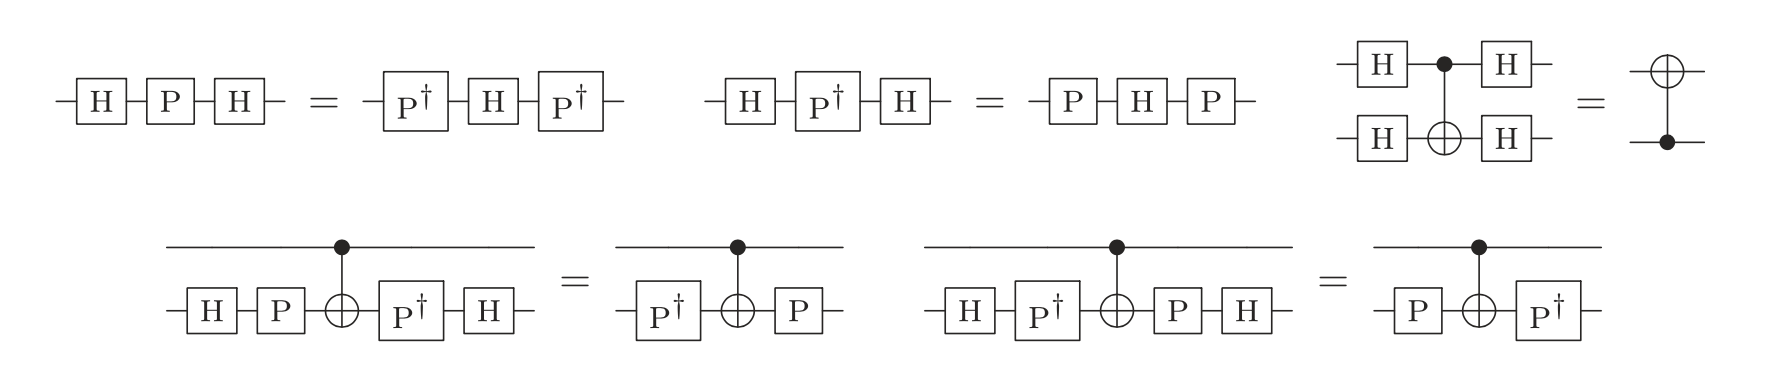
\includegraphics[width=0.9\linewidth]{images/hardmard_reduction.png}
            \caption{Subcircuit patterns in Hardmard Reduction}
        \end{figure}
    \end{center}

    \subsubsection{Gate Cancellation}
    When a pair of conjugate transpose gates are adjacent, they can both be cancelled.

    In this section, we implement gate cancellation for $RZ$ gate, we traverse all $RZ$ gates and try to move it by swap with adjacent commutative subcircuit if posible (we only consider serveral  built-in commutation rules (\ref{commutation}) since it is hard to determine whether two gates are commutative) until encountering its conjugate transpose or reaching endpoints of the circuit.

    \begin{center}
        \begin{figure}
            \label{commutation}
            \centering
            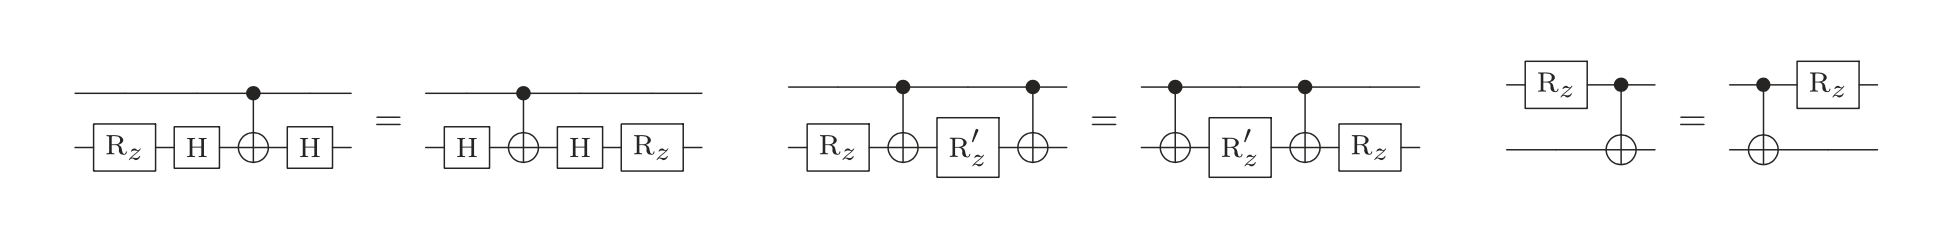
\includegraphics[width=0.9\linewidth]{images/gate_cancellation.png}
            \caption{Commutation rules for RZ gate}
        \end{figure}
    \end{center}



\section{Usage and Examples}

See the \texttt{readme} file of our repository for code structure and usage.
Here we give some examples of $\lambda_Q$ program.
Note that a $\lambda_Q$ program should contain at least one circuit abstraction (i.e. $\kappa$ abstraction) as its entry point, just like the main function in other programming languages.
For simplicity, we assume the last circuit abstraction is the entry point.


\subsection{Quantum Teleportation}

This is a classical example also appeared in some other papers about quantum programming languages.
It can be written in $\lambda_Q$ like follows.

\begin{lstlisting}[language=Lambda]
fun bell00 = / () : One .
  a <- gate init0 ();
  b <- gate init0 ();
  a <- gate H a;
  (a, b) <- gate CNOT (a, b);
  output (a, b)

fun alice = / (q, a) : Qubit # Qubit .
  (q, a) <- gate CNOT (q, a);
  q <- gate H q;
  x <- gate meas q;
  y <- gate meas a;
  output (x,y)

fun bob = / ((w1, w2), q) : Bit # Bit # Qubit .
    (x1, x2) <-| lift (w1, w2);
    q <- capp (if x2
               then (/ t : Qubit . gate X t)
               else (/ t : Qubit . output t)
         ) to q;
    capp (if x1
          then (/ t : Qubit . gate Z t)
          else (/ t : Qubit . output t)
    ) to q

fun teleport = / () : One .
  q <- gate init0 ();
  (a, b) <- capp bell00 to ();
  (x, y) <- capp alice to (q, a);
  capp bob to ((x, y), b);
\end{lstlisting}

The output of the frontend is:
\begin{lstlisting}[language=lambda]
openqasm 2.0;
qreg r0[1];
qreg r1[1];
qreg r2[1];
H r1;
CX r1, r2;
CX r0, r1;
H r0;
creg r3[1];
measure r0 -> r3;
creg r4[1];
measure r1 -> r4;
if (r4 == 1) X r2;
if (r3 == 1) Z r2;
\end{lstlisting}

And the output of the backend is:
\begin{lstlisting}[language=lambda]
openqasm 2.0;
qreg q[3];
H q[1];
CX q[1], q[2];
CX q[0], q[1];
H q[0];
creg r3[1];
measure q[0]->r3;
creg r4[1];
measure q[1]->r4;
if(r4 == 1) X q[2];
if(r3 == 1) Z q[2];
\end{lstlisting}

There is not too much difference between IR and output because this quantum does not fit any optimization.

\subsection{Simple Optimization}
Here is another simple example to show the optimization power of our backend.
The original $\lambda_Q$ program is:
\begin{lstlisting}[language=lambda]
fun qwq = / () : One .
  a <- gate init0 ();
  b <- gate init0 ();
  a <- gate H a;
  b <- gate H b;
  (c, d) <- gate CNOT (a, b);
  c <- gate H c;
  d <- gate H d;
  output (c, d)
\end{lstlisting}

The output of the frontend is:
\begin{lstlisting}[language=lambda]
openqasm 2.0;
qreg r0[1];
qreg r1[1];
H r0;
H r1;
CX r0, r1;
H r0;
H r1;
\end{lstlisting}

And the output of the backend is:
\begin{lstlisting}[language=lambda]
openqasm 2.0;
qreg q[2];
CX q[1], q[0];
\end{lstlisting}

The optimization really works!


\section{Roles and Responsibilities}
Wenhao Tang:
\begin{itemize}
  \item $\lambda_Q$ language design;
  \item Implementation of Frontend;
\end{itemize}

\noindent Xinzhao Wang:
\begin{itemize}
  \item Implementation of Backend;
\end{itemize}
\mycomment{twh}{Supplement here @wxz.}

\medskip

\bibliography{reference}

\end{document}